
\documentclass[12pt]{article}
\usepackage[utf8]{inputenc}
\usepackage{upquote}
\usepackage[margin=20mm]{geometry} 
\usepackage{amsmath,amsthm,amssymb}
\usepackage{graphicx}
\usepackage{listings}
\newenvironment{statement}[2][Statement]{\begin{trivlist}
\item[\hskip \labelsep {\bfseries #1}\hskip \labelsep {\bfseries #2.}]}{\end{trivlist}}
\usepackage{xcolor}

\usepackage{subfigure}


% Listings package for code rendering (No external dependencies)
\usepackage{listings}  
\usepackage{xcolor}   % Color support
\usepackage{tcolorbox} % Box for better appearance

% Define custom colors for code highlighting
\definecolor{codegreen}{rgb}{0,0.6,0}
\definecolor{codegray}{rgb}{0.5,0.5,0.5}
\definecolor{codepurple}{rgb}{0.58,0,0.82}
\definecolor{backcolour}{rgb}{0.95,0.95,0.92}


\lstset{frame=tb,
    language=Python,
    backgroundcolor=\color{backcolour},   
    commentstyle=\color{codegreen},
    keywordstyle=\color{magenta},
    numberstyle=\tiny\color{codegray},
    stringstyle=\color{codepurple},
    basicstyle=\ttfamily\footnotesize,
    breakatwhitespace=false,         
    breaklines=true,                 
    keepspaces=true,                 
    numbers=left,       
    numbersep=5pt,                  
    showspaces=false,                
    showstringspaces=false,
    showtabs=false,                  
    tabsize=2,
}





\title{Assignment 5}


\author{Author \\
 Wanjing Hu / fng685@alumni.ku.dk  \\
 Shuangcheng Jia / bkg713@alumni.ku.dk/   \\
 Zhigao Yan / sxd343@alumni.ku.dk  \\
} 

\begin{document}
\maketitle

\section{Inspecting Spectrograms}
%Shuangcheng
\section{Inverse filtering}
%zhigao

\section{Fixed scale feature detectors}

%Wanjing
\subsection{}

\textbf{sigma}: This is the Standard deviation of the Gaussian filter, controlling Gaussian smoothing. Higher sigma (e.g., 3) reduces noise but blurs edges, leading to thicker and fewer edges.

\textbf{low\_threshold/high\_threshold}: These two parameters determine edge connectivity. Lower thresholds (e.g., 0.05/0.2) detect more edges, including noise, while higher thresholds retain only strong edges.

\begin{lstlisting}
image = skimage.io.imread('../TestImages/Week 1/hand.tiff', as_gray=True)
edges_default = skimage.feature.canny(image)
edges_sigma3 = skimage.feature.canny(image, sigma=3)
edges_low_high = skimage.feature.canny(image, low_threshold=0.05, high_threshold=0.2)
\end{lstlisting}

\begin{figure}[h]
    \centering
    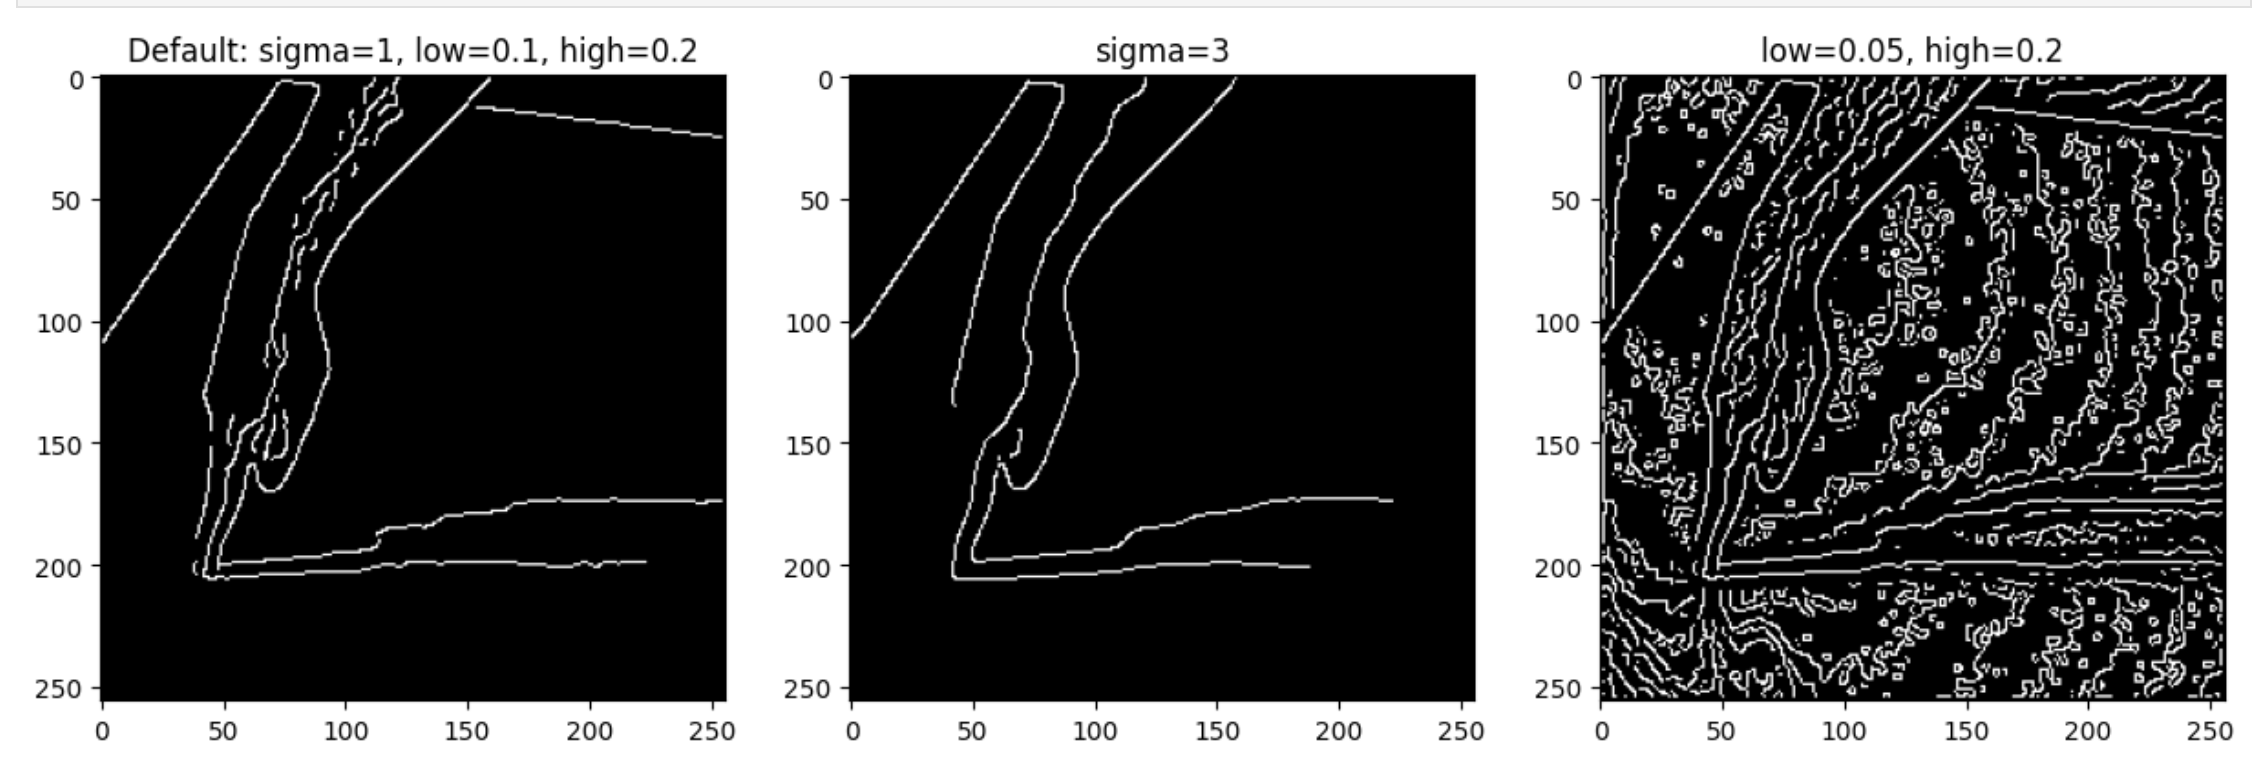
\includegraphics[width=0.6\textwidth]{pics/a5-3.1} 
    \caption{xx.}
\end{figure}

\subsection{}

\textbf{sigma}: Larger sigma (e.g., 3) smooths gradients, detecting corners at a coarser scale.

\textbf{k}: Higher k (e.g., 0.2) reduces false corners but may miss weaker ones.

\textbf{Method eps}: Uses Noble’s corner measure. The lower the eps is, the more sensitive the corner decection is.

\begin{lstlisting}
image_house = skimage.io.imread('../TestImages/Week 1/modelhouses.png', as_gray=True)

harris1 = 
	skimage.feature.corner_harris(image_house, sigma=1, k=0.05, method='k')
harris2 = 
	skimage.feature.corner_harris(image_house, sigma=3, k=0.05, method='k')
harris3 = 
	skimage.feature.corner_harris(image_house, sigma=1, k=0.2, method='k')
harris4 = 
	skimage.feature.corner_harris(image_house, sigma=1, method='eps', eps=0.01)

fig, axes = plt.subplots(2, 2, figsize=(10, 10))
axes[0,0].imshow(harris1, cmap='viridis')
axes[0,0].set_title('sigma=1, k=0.05')
axes[0,1].imshow(harris2, cmap='viridis')
axes[0,1].set_title('sigma=3, k=0.05')
axes[1,0].imshow(harris3, cmap='viridis')
axes[1,0].set_title('sigma=1, k=0.2')
axes[1,1].imshow(harris4, cmap='viridis')
axes[1,1].set_title('sigma=1, eps=0.01')
plt.show()
\end{lstlisting}

\begin{figure}[h]
    \centering
    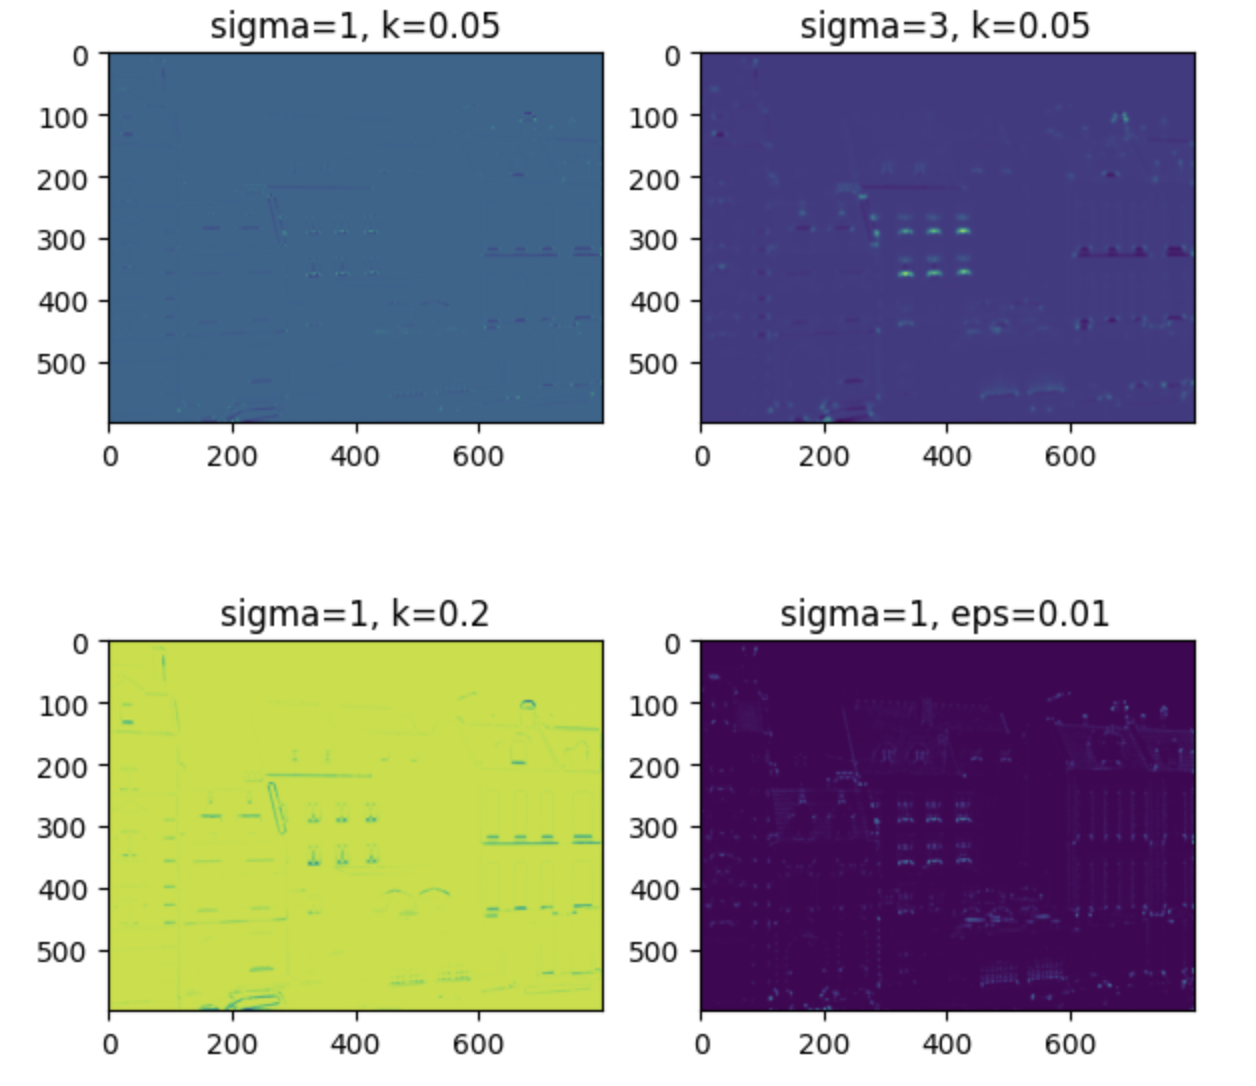
\includegraphics[width=0.6\textwidth]{pics/a5-3.2} 
    \caption{xx.}
\end{figure}

\subsection{}

The figure shows the 250 strongest Harris corners (red crosses) detected on modelhouses.png using parameters sigma=1, k=0.05, and min\_distance=1. Corners are localized at building edges and intersections.

\begin{lstlisting}
def find_harris_corners(image, sigma=1, k=0.05, method='k', min_distance=1, num_peaks=250):
    from skimage.feature import corner_harris, corner_peaks
    response = corner_harris(image, sigma=sigma, k=k, method=method)
    coords = corner_peaks(response, min_distance=min_distance, num_peaks=num_peaks)
    return coords

coords = find_harris_corners(image_house, sigma=1, k=0.05)
\end{lstlisting}

\begin{figure}[h]
    \centering
    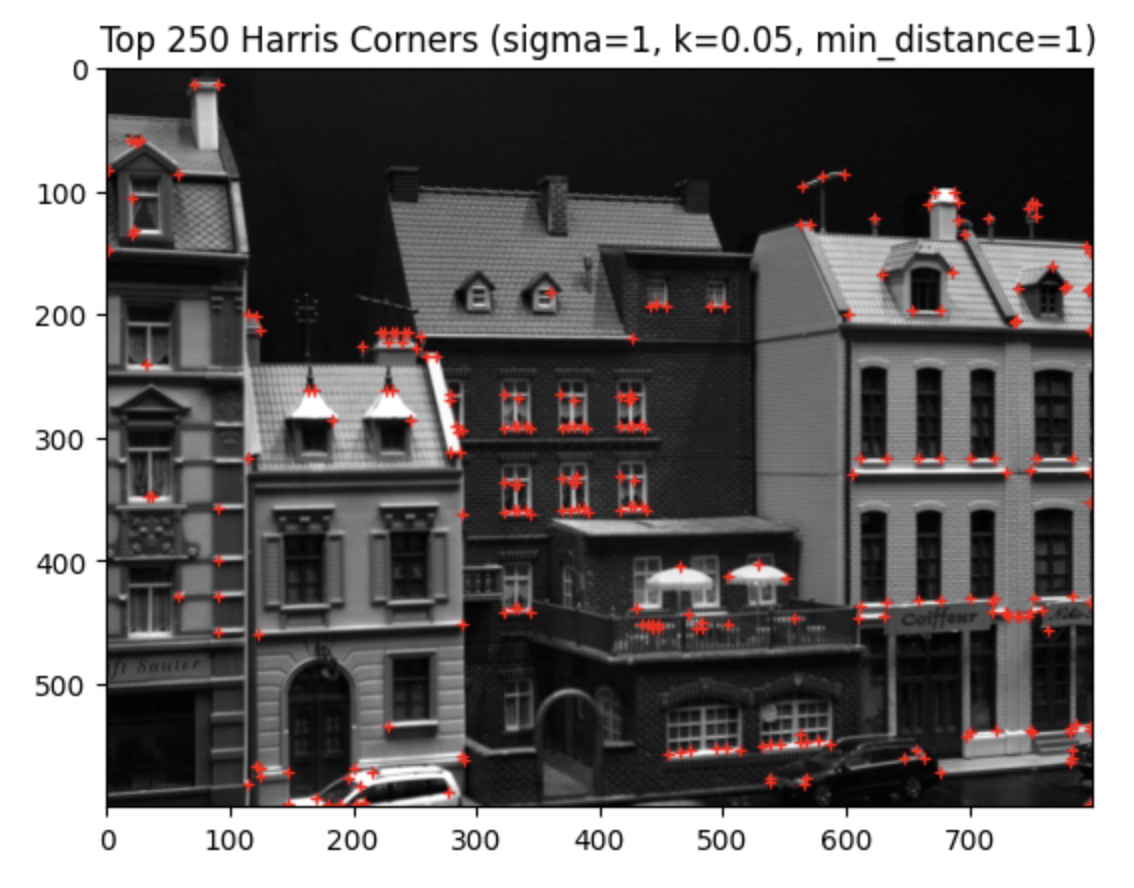
\includegraphics[width=0.6\textwidth]{pics/a5-3.3} 
    \caption{xx.}
\end{figure}

\section{Scale-space blob detector}
%Shuangcheng1
\subsection{}
The following code demonstrates the convolution property of 2D Gaussian functions by generating, convolving, and comparing Gaussian blob images:
\begin{lstlisting}[caption={Code for 4.1},captionpos=b]
# 1. Define the 2D Gaussian function
def gaussian(x, y, sigma):
    return (1 / (2 * np.pi * sigma**2)) * np.exp(-(x**2 + y**2) / (2 * sigma**2))
# 2. Generate a blob image using the Gaussian function
def model_blob_image(x, y, sigma): return gaussian(x, y, sigma)
# 3. Apply Gaussian convolution to the blob image
def convolve_blob_image(original_blob, gaussian_filter):
    return convolve2d(original_blob, gaussian_filter, mode='same')

grid_size = 30
x = np.arange(-grid_size // 2, grid_size // 2 + 1)
y = np.arange(-grid_size // 2, grid_size // 2 + 1)
x_coords, y_coords = np.meshgrid(x, y)

# Generate the initial blob image with sigma = 1
sigma = 1
blob_image_original = model_blob_image(x_coords, y_coords, sigma)

# Generate the Gaussian filter for convolution with tau = 2
tau = 2
gaussian_filter = model_blob_image(x_coords, y_coords, tau)

blob_image_convolved = convolve_blob_image(blob_image_original, gaussian_filter)

gamma = np.sqrt(sigma**2 + tau**2)
blob_image_calculated = model_blob_image(x_coords, y_coords, gamma)

difference_image = blob_image_calculated - blob_image_convolved

## The visualization part is not described here.

\end{lstlisting}

\FloatBarrier

\begin{figure}[ht]
    \centering
    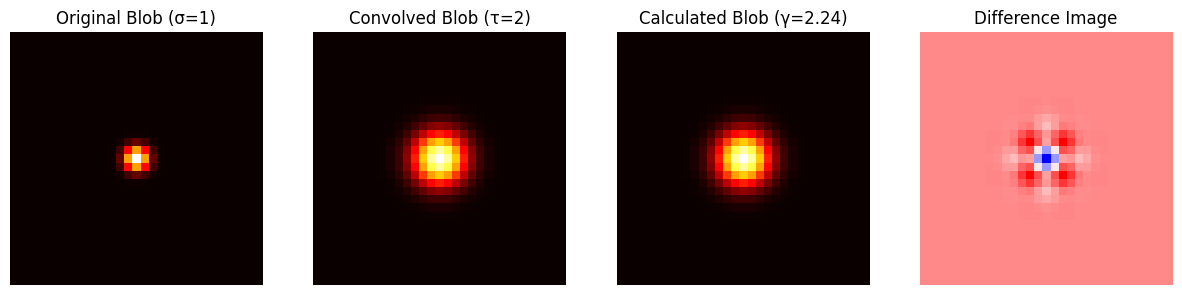
\includegraphics[width=1.0\columnwidth, keepaspectratio]{pics/a5-4.1.png}
    \caption[]{Result for 4.1}
    \label{fig:4.1}
\end{figure}

\FloatBarrier
To verify the convolution property of two-dimensional Gaussian functions:
    $G(x,y,\sigma) * G(x,y,\tau) = G(x,y, \sqrt{\sigma^2 + \tau^2}),
$
we construct and visualize different Gaussian blob images to confirm this property.

Figure \ref{fig:4.1} presents the results. The first subplot shows the original blob image with scale $\sigma = 1$. The second subplot from the left is the convolved blob image, obtained by applying a Gaussian filter with scale $\tau = 2$ to the original blob. The third subplot is the calculated blob image, generated directly using a Gaussian function with scale $\gamma = \sqrt{\sigma^2 + \tau^2} \approx 2.24$. The last subplot shows the difference image, computed as the calculated blob image minus the convolved blob image.

From the difference image, we observe that the center region is dark, indicating that the convolved blob image has slightly lower pixel values than the calculated blob image due to Gaussian smoothing. The edges of the central region are relatively bright, meaning the convolved image has higher pixel values in those areas, likely due to intensity spread during convolution. These differences arise from numerical approximations and edge effects but do not contradict the theoretical formulation.

The results confirm that convolving a Gaussian function with another Gaussian produces a new Gaussian with an increased standard deviation as predicted by the convolution theorem.

\subsection{}
The two-dimensional Gaussian function is:
\begin{equation}
    G(x,y,\sigma) = \frac{1}{2\pi\sigma^2} \exp\left(-\frac{x^2 + y^2}{2\sigma^2} \right).
\end{equation}
Taking its Fourier transform:
\begin{equation}
    \mathcal{F} \{ G(x,y,\sigma) \} = \exp\left(-\frac{1}{2} \sigma^2 (k_x^2 + k_y^2) \right).
\end{equation}
This shows that the Fourier transform of a Gaussian remains a Gaussian in frequency space.
Next, the convolution theorem states that the Fourier transform of a convolution is the product of the individual Fourier transforms:
\begin{equation}
    \mathcal{F} \{ G(x,y,\sigma) * G(x,y,\tau) \} = \mathcal{F} \{ G(x,y,\sigma) \} \cdot \mathcal{F} \{ G(x,y,\tau) \}.
\end{equation}
Substituting the Gaussian Fourier transforms:
\begin{equation}
    \exp\left(-\frac{1}{2} \sigma^2 (k_x^2 + k_y^2) \right) \cdot \exp\left(-\frac{1}{2} \tau^2 (k_x^2 + k_y^2) \right).
\end{equation}
Using exponent addition:
\begin{equation}
    \exp\left(-\frac{1}{2} (\sigma^2 + \tau^2) (k_x^2 + k_y^2) \right).
\end{equation}
This is the Fourier transform of a Gaussian with standard deviation:
\begin{equation}
    \sqrt{\sigma^2 + \tau^2}.
\end{equation}
Since the inverse Fourier transform of this expression is again a Gaussian with the updated standard deviation, we conclude:
\begin{equation}
    G(x,y,\sigma) * G(x,y,\tau) = G(x,y,\sqrt{\sigma^2 + \tau^2}).
\end{equation}

\subsection{}
\begin{enumerate}[label=\roman*., leftmargin=1cm]
    \item
We aim to derive the closed-form expression for the scale-normalized Laplacian:

\begin{equation}
    H(x,y,\tau) = I_{xx}(x,y,\tau) + I_{yy}(x,y,\tau).
\end{equation}

From the definition of scale-normalized derivatives:
\begin{equation}
    I_{x^m y^n}(x, y, \tau) = \tau^{\gamma(m+n)} \frac{\partial^{m+n} I(x,y,\tau)}{\partial x^m \partial y^n},
\end{equation}
set \( \gamma = 1 \), we obtain:
\begin{equation}
    I_{xx}(x,y,\tau) = \tau^2 \frac{\partial^2 I(x,y,\tau)}{\partial x^2}, \quad
    I_{yy}(x,y,\tau) = \tau^2 \frac{\partial^2 I(x,y,\tau)}{\partial y^2}.
\end{equation}
Thus, the scale-normalized Laplacian is:
\begin{equation}
    H(x,y,\tau) = \tau^2 \left( \frac{\partial^2 I(x,y,\tau)}{\partial x^2} + \frac{\partial^2 I(x,y,\tau)}{\partial y^2} \right).
\end{equation}
Use the convolution property of Gaussians:
\begin{equation}
    I(x,y,\tau) = G(x,y,\sigma) * G(x,y,\tau) = G(x,y,\sqrt{\sigma^2 + \tau^2}),
\end{equation}
Express it as:
\begin{equation}
    I(x,y,\tau) = \frac{1}{2\pi(\sigma^2 + \tau^2)} e^{-\frac{x^2 + y^2}{2(\sigma^2 + \tau^2)}}.
\end{equation}
Use the known formula for the second derivative of a Gaussian:
\begin{equation}
    \frac{\partial^2 I}{\partial x^2} = - \left(\frac{1}{2\pi (\sigma^2 + \tau^2)^2}\right) \left(1 - \frac{x^2}{\sigma^2 + \tau^2} \right) e^{-\frac{x^2 + y^2}{2(\sigma^2 + \tau^2)}},
\end{equation}
and similarly for \( y \):
\begin{equation}
    \frac{\partial^2 I}{\partial y^2} = - \left(\frac{1}{2\pi (\sigma^2 + \tau^2)^2}\right) \left(1 - \frac{y^2}{\sigma^2 + \tau^2} \right) e^{-\frac{x^2 + y^2}{2(\sigma^2 + \tau^2)}}.
\end{equation}
Sum both derivatives:
\begin{equation}
    \frac{\partial^2 I}{\partial x^2} + \frac{\partial^2 I}{\partial y^2} = - \left(\frac{1}{2\pi (\sigma^2 + \tau^2)^2}\right) \left(2 - \frac{x^2 + y^2}{\sigma^2 + \tau^2} \right) e^{-\frac{x^2 + y^2}{2(\sigma^2 + \tau^2)}}.
\end{equation}
Multiplying by \( \tau^2 \), we obtain:
\begin{equation}
    H(x,y,\tau) = - \left( \frac{\tau^2}{2\pi (\sigma^2 + \tau^2)^2} \right) \left(2 - \frac{x^2 + y^2}{\sigma^2 + \tau^2} \right) e^{-\frac{x^2 + y^2}{2(\sigma^2 + \tau^2)}}.
\end{equation}
    \item
    At the point \( (0,0) \), the scale-normalized Laplacian is given by
\begin{equation}
    H(0,0,\tau) = -\frac{\tau^2}{\pi (\sigma^2 + \tau^2)^2}.
\end{equation}

To find the extremal points, we differentiate with respect to \( \tau \):
\begin{equation}
    \frac{dH}{d\tau} = \frac{4\tau^3}{\pi (\sigma^2 + \tau^2)^3} - \frac{2\tau}{\pi (\sigma^2 + \tau^2)^2}.
\end{equation}

Setting \( \frac{dH}{d\tau} = 0 \), we factor out \( \tau \), obtaining the solutions
\begin{equation}
    \tau = 0, \quad \tau = \pm\sigma.
\end{equation}

To classify these points, we compute the second derivative:
\begin{equation}
    \frac{d^2H}{d\tau^2} = -\frac{24\tau^4}{\pi (\sigma^2 + \tau^2)^4} + \frac{20\tau^2}{\pi (\sigma^2 + \tau^2)^3} - \frac{2}{\pi (\sigma^2 + \tau^2)^2}.
\end{equation}

Evaluating at \( \tau = 0 \), we get
\begin{equation}
    \frac{d^2H}{d\tau^2} \Big|_{\tau=0} = -\frac{2}{\pi \sigma^4} < 0,
\end{equation}
indicating a maximum. For \( \tau = \pm\sigma \),
\begin{equation}
    \frac{d^2H}{d\tau^2} \Big|_{\tau = \pm \sigma} = \frac{1}{2\pi \sigma^4} > 0,
\end{equation}
indicating minima.

Thus, \( H(0,0,\tau) \) has a maximum at \( \tau = 0 \) and minima at \( \tau = \pm\sigma \). There are no saddle points.

    \item
Figure \ref{fig:4.3} shows \( H(0,0,\tau) \) as a function of \( \tau \), with vertical dashed lines marking \( \tau = 1,2,3 \) and their negatives.

    \FloatBarrier

\begin{figure}[ht]
    \centering
    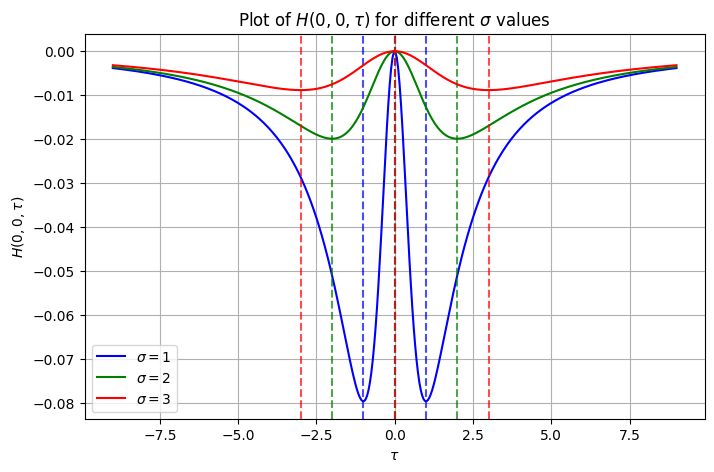
\includegraphics[width=0.7\columnwidth, keepaspectratio]{pics/a5-4.3.png}
    \caption[]{Figure for 4.3}
    \label{fig:4.3}
\end{figure}

\FloatBarrier

The function reaches a maximum at \( \tau = 0 \), confirming our analysis. The minima occur at \( \tau = \pm\sigma \) (here, \( \sigma = 1 \)), consistent with theoretical predictions. The dashed lines highlight different scales where \( H(0,0,\tau) \) is evaluated. As \( \tau \) increases, \( H(0,0,\tau) \) approaches zero, indicating reduced response at large scales.

This confirms that \( H(0,0,\tau) \) has a peak at \( \tau = 0 \) and dips at characteristic scales, with no saddle points.
\end{enumerate}

\subsection{}
The code shows the blob detection based on the scale-normalized Laplacian of Gaussian (LoG).
\begin{lstlisting}[caption={Code for 4.4},captionpos=b]
## Defining parameters part is omitted here

# Compute the scale-normalized Laplacian and detect extrema
for sigma in sigma_values:
    H = sigma**(2 * gamma)*(gaussian_filter(image, sigma=sigma, order=(2, 0)) +
                            gaussian_filter(image, sigma=sigma, order=(0, 2)))

    # Detect local maxima and minima
    maxima = feature.peak_local_max(H, min_distance=10, threshold_abs=0.02, exclude_border=False)
    minima = feature.peak_local_max(-H, min_distance=5, threshold_abs=0.01, exclude_border=False)

    # Store detected points with their scale
    for y, x in maxima:
        blobs.append((y, x, sigma, H[y, x]))
    for y, x in minima:
        blobs.append((y, x, sigma, H[y, x]))

# Sort blobs by absolute response value and select the strongest
blobs.sort(key=lambda b: -abs(b[3]))
blobs_maxima = blobs[:num_blobs]
blobs_minima = blobs[-num_blobs:]

## The visualization part is not described here.

\end{lstlisting}

Fig \ref{fig:4.4} illustrates the detection results on the sunflower.tiff image.


\FloatBarrier

\begin{figure}[ht]
    \centering
    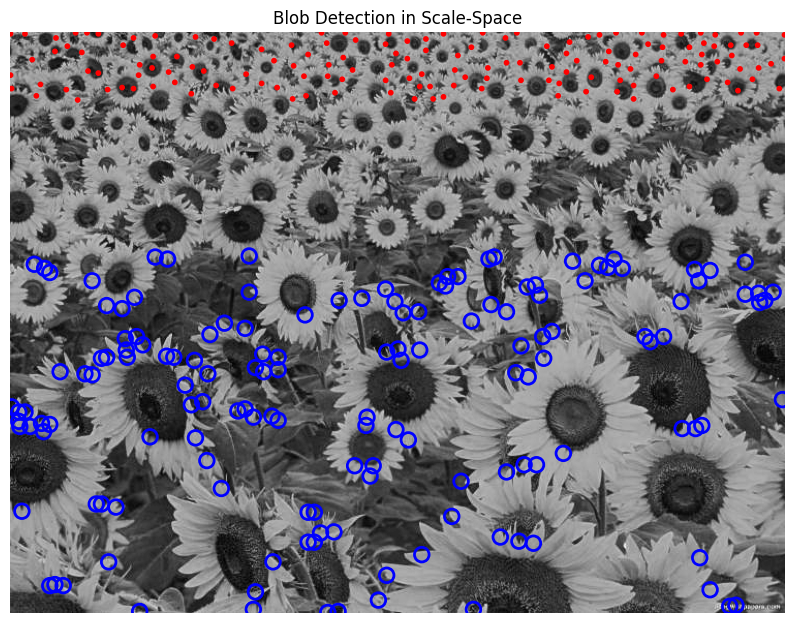
\includegraphics[width=0.7\columnwidth, keepaspectratio]{pics/a5-4.4.png}
    \caption[]{Result for 4.4}
    \label{fig:4.4}
\end{figure}

\FloatBarrier

Maxima of \( H(x,y,\tau) \) represent bright blob-like structures in the image, corresponding to regions that are brighter than their surroundings, such as the bright petals of the sunflowers or the sky. Minima of \( H(x,y,\tau) \) represent dark blob-like structures, corresponding to regions that are darker than their surroundings, such as the dark centers of the sunflowers.

Thus, maxima highlight bright object regions, while minima emphasize dark object regions.

\end{document}
